\documentclass[conference]{IEEEtran}

\usepackage{cite}
\usepackage{url}
\usepackage[cmex10]{amsmath}
\usepackage{amssymb}
\usepackage{multirow}
\interdisplaylinepenalty=2500

% *** GRAPHICS RELATED PACKAGES ***
%

% % % % % MACROS  % % % % % % %
\newcommand{\imagepath}{../../images/external/location_routing}
\newcommand{\colwidth}{2.6in}
% % % % % % % % % % % % % % % %

\ifCLASSINFOpdf
  \usepackage[pdftex]{graphicx}
  % declare the path(s) where your graphic files are
  % ../.. is the GeocronDocuments directory
  \graphicspath{{../../images/external/location_routing}{../../images/}}
  % and their extensions so you won't have to specify these with
  % every instance of \includegraphics
  \DeclareGraphicsExtensions{.pdf,.png}
\else
  % or other class option (dvipsone, dvipdf, if not using dvips). graphicx
  % will default to the driver specified in the system graphics.cfg if no
  % driver is specified.
  % \usepackage[dvips]{graphicx}
  % declare the path(s) where your graphic files are
  % \graphicspath{{../eps/}}
  % and their extensions so you won't have to specify these with
  % every instance of \includegraphics
  % \DeclareGraphicsExtensions{.eps}
\fi



% *** SPECIALIZED LIST PACKAGES ***
%
%\usepackage{algpseudocode}
% algorithmic.sty was written by Peter Williams and Rogerio Brito.
% This package provides an algorithmic environment fo describing algorithms.
% You can use the algorithmic environment in-text or within a figure
% environment to provide for a floating algorithm. Do NOT use the algorithm
% floating environment provided by algorithm.sty (by the same authors) or
% algorithm2e.sty (by Christophe Fiorio) as IEEE does not use dedicated
% algorithm float types and packages that provide these will not provide
% correct IEEE style captions. The latest version and documentation of
% algorithmic.sty can be obtained at:
% http://www.ctan.org/tex-archive/macros/latex/contrib/algorithms/
% There is also a support site at:
% http://algorithms.berlios.de/index.html
% Also of interest may be the (relatively newer and more customizable)
% algorithmicx.sty package by Szasz Janos:
% http://www.ctan.org/tex-archive/macros/latex/contrib/algorithmicx/




% *** ALIGNMENT PACKAGES ***
%
%\usepackage{array}
% Frank Mittelbach's and David Carlisle's array.sty patches and improves
% the standard LaTeX2e array and tabular environments to provide better
% appearance and additional user controls. As the default LaTeX2e table
% generation code is lacking to the point of almost being broken with
% respect to the quality of the end results, all users are strongly
% advised to use an enhanced (at the very least that provided by array.sty)
% set of table tools. array.sty is already installed on most systems. The
% latest version and documentation can be obtained at:
% http://www.ctan.org/tex-archive/macros/latex/required/tools/


%\usepackage{mdwmath}
%\usepackage{mdwtab}
% Also highly recommended is Mark Wooding's extremely powerful MDW tools,
% especially mdwmath.sty and mdwtab.sty which are used to format equations
% and tables, respectively. The MDWtools set is already installed on most
% LaTeX systems. The lastest version and documentation is available at:
% http://www.ctan.org/tex-archive/macros/latex/contrib/mdwtools/


% IEEEtran contains the IEEEeqnarray family of commands that can be used to
% generate multiline equations as well as matrices, tables, etc., of high
% quality.


%\usepackage{eqparbox}
% Also of notable interest is Scott Pakin's eqparbox package for creating
% (automatically sized) equal width boxes - aka "natural width parboxes".
% Available at:
% http://www.ctan.org/tex-archive/macros/latex/contrib/eqparbox/





% *** SUBFIGURE PACKAGES ***
%\usepackage[tight,footnotesize]{subfigure}
% subfigure.sty was written by Steven Douglas Cochran. This package makes it
% easy to put subfigures in your figures. e.g., "Figure 1a and 1b". For IEEE
% work, it is a good idea to load it with the tight package option to reduce
% the amount of white space around the subfigures. subfigure.sty is already
% installed on most LaTeX systems. The latest version and documentation can
% be obtained at:
% http://www.ctan.org/tex-archive/obsolete/macros/latex/contrib/subfigure/
% subfigure.sty has been superceeded by subfig.sty.



% subfig.sty, also written by Steven Douglas Cochran, is the modern
% replacement for subfigure.sty. However, subfig.sty requires and
% automatically loads Axel Sommerfeldt's caption.sty which will override
% IEEEtran.cls handling of captions and this will result in nonIEEE style
% figure/table captions. To prevent this problem, be sure and preload
% caption.sty with its "caption=false" package option. This is will preserve
% IEEEtran.cls handing of captions. Version 1.3 (2005/06/28) and later 
% (recommended due to many improvements over 1.2) of subfig.sty supports
% the caption=false option directly:
\usepackage[caption=false,font=footnotesize]{subfig}
%
% The latest version and documentation can be obtained at:
% http://www.ctan.org/tex-archive/macros/latex/contrib/subfig/
% The latest version and documentation of caption.sty can be obtained at:
% http://www.ctan.org/tex-archive/macros/latex/contrib/caption/




% *** FLOAT PACKAGES ***
%
%\usepackage{fixltx2e}
% fixltx2e, the successor to the earlier fix2col.sty, was written by
% Frank Mittelbach and David Carlisle. This package corrects a few problems
% in the LaTeX2e kernel, the most notable of which is that in current
% LaTeX2e releases, the ordering of single and double column floats is not
% guaranteed to be preserved. Thus, an unpatched LaTeX2e can allow a
% single column figure to be placed prior to an earlier double column
% figure. The latest version and documentation can be found at:
% http://www.ctan.org/tex-archive/macros/latex/base/



%\usepackage{stfloats}
% stfloats.sty was written by Sigitas Tolusis. This package gives LaTeX2e
% the ability to do double column floats at the bottom of the page as well
% as the top. (e.g., "\begin{figure*}[!b]" is not normally possible in
% LaTeX2e). It also provides a command:
%\fnbelowfloat
% to enable the placement of footnotes below bottom floats (the standard
% LaTeX2e kernel puts them above bottom floats). This is an invasive package
% which rewrites many portions of the LaTeX2e float routines. It may not work
% with other packages that modify the LaTeX2e float routines. The latest
% version and documentation can be obtained at:
% http://www.ctan.org/tex-archive/macros/latex/contrib/sttools/
% Documentation is contained in the stfloats.sty comments as well as in the
% presfull.pdf file. Do not use the stfloats baselinefloat ability as IEEE
% does not allow \baselineskip to stretch. Authors submitting work to the
% IEEE should note that IEEE rarely uses double column equations and
% that authors should try to avoid such use. Do not be tempted to use the
% cuted.sty or midfloat.sty packages (also by Sigitas Tolusis) as IEEE does
% not format its papers in such ways.

\hyphenation{op-tical net-works semi-conduc-tor}


\begin{document}
%
% can use linebreaks \\ within to get better formatting as desired
\title{A Survey of Location-Based Routing Techniques}

\author{\IEEEauthorblockN{Kyle E. Benson and Zhipeng Huang}
\IEEEauthorblockA{Donald Bren School of Information and Computer Sciences\\
University of California, Irvine\\
Irvine, California 92697\\
Email: kebenson@uci.edu, zhipengh@uci.edu}}

% use for special paper notices
\IEEEspecialpapernotice{(Survey Paper for CS 237 - Distributed Systems Middleware)}


\maketitle



\begin{abstract}
In this survey paper, we categorize and present various techniques for routing with location information.
These strategies are applied in various types of networks, including sensor, mobile ad-hoc, and even wired networks.
We present the motivations for these routing protocols and their evolution over time, such as how certain categories were developed in response to limitations of previous ones.
\end{abstract}

% For peer review papers, you can put extra information on the cover
% page as needed:
% \ifCLASSOPTIONpeerreview
% \begin{center} \bfseries EDICS Category: 3-BBND \end{center}
% \fi
%
% For peerreview papers, this IEEEtran command inserts a page break and
% creates the second title. It will be ignored for other modes.
\IEEEpeerreviewmaketitle



\section{Introduction}

Traditional network routing typically relies on a static addressing scheme: in order to contact a node, say $B$, the sending node, say $A$, must know some unique identifier associated with $B$ in order to send a message to it.
Some communication paradigms, such as multicast and broadcast, relax this assumption by communicating with entire groups, nodes belonging to a specific group identifier and all nodes in a network, respectively.
In order to route these messages, intermediate nodes must know the next hop along the path to $B$.
This requires knowledge of the network topology, either partial or full.
Protocols to establish this knowledge typically include link-state (knowledge of full paths) or distance-vector (knowledge of the next hop towards a given destination) algorithms, although others exist such as label-switching, which requires preconfiguring labels to correspond to particular paths, interfaces, etc.

However, one can imagine situations in which maintaining knowledge of the network topology may be unfeasible, such as mobile ad-hoc networks (MANETs), where the nodes are constantly moving. To maintain traditional routing protocols would be a rather difficult task under MANETs. For link-state protocols, the state update message flooding would simply paralyze the MANET, on the other hand distance-vector algorithms may not even work since the next hop may not even be there in the next moment. For wireless networks like MANETs, how to maintain a routing scheme that has lower overheads, could converge in constant time, and overcome the inherent problem introduced by wireless network itself such as high loss rate, is a huge challenge.

Moreover, it is not only the newly fledged wireless network but also the long existing wired network need a new thinking on routing. For wired networks, how to cope with emergency situation like link failure happens when earthquake or tsunami occurs. It takes long hours and high labor cost for current routing protocols to recover from failure. Black spots in the abstract routing topology may not be easily detected and the reconstruction of the network topology could be still error-prone.

Therefore it is important to investigate new routing designs like location-based routing techniques to keep up with the challenge. In this survey paper, we have looked into various areas regarding location-based routing, and categorized those routing techniques in different areas into the following sections: Location Service,  Greedy Forwarding, Trajectory-based routing, Zone Forwarding (Agent/Agent-less),   Geometric Routing, Clustering. The conclusion of this survey is provided at the end of this paper.


% % % % % % % % % % % % % % % % % % % % % % % % % % % % % % % % % % % % % % % % % %

\section{Location Service}

Before a source node can route to a destination by location information, it must obviously possess this data.
It may not be feasible for every node in a larger network to maintain the whereabouts of every other node, especially since these may change if nodes are mobile.
To address this issue, a location routing system must provide a mechanism for scalably querying node updated locations.
Typically, these mechanisms use hierarchical and/or tree-based approaches to make full advantage of the asymptotic properties of such structures, such as completing queries in O(logn) hops (where n $=$ the network size).

\begin{figure}
\label{fig:location-service}
\centering
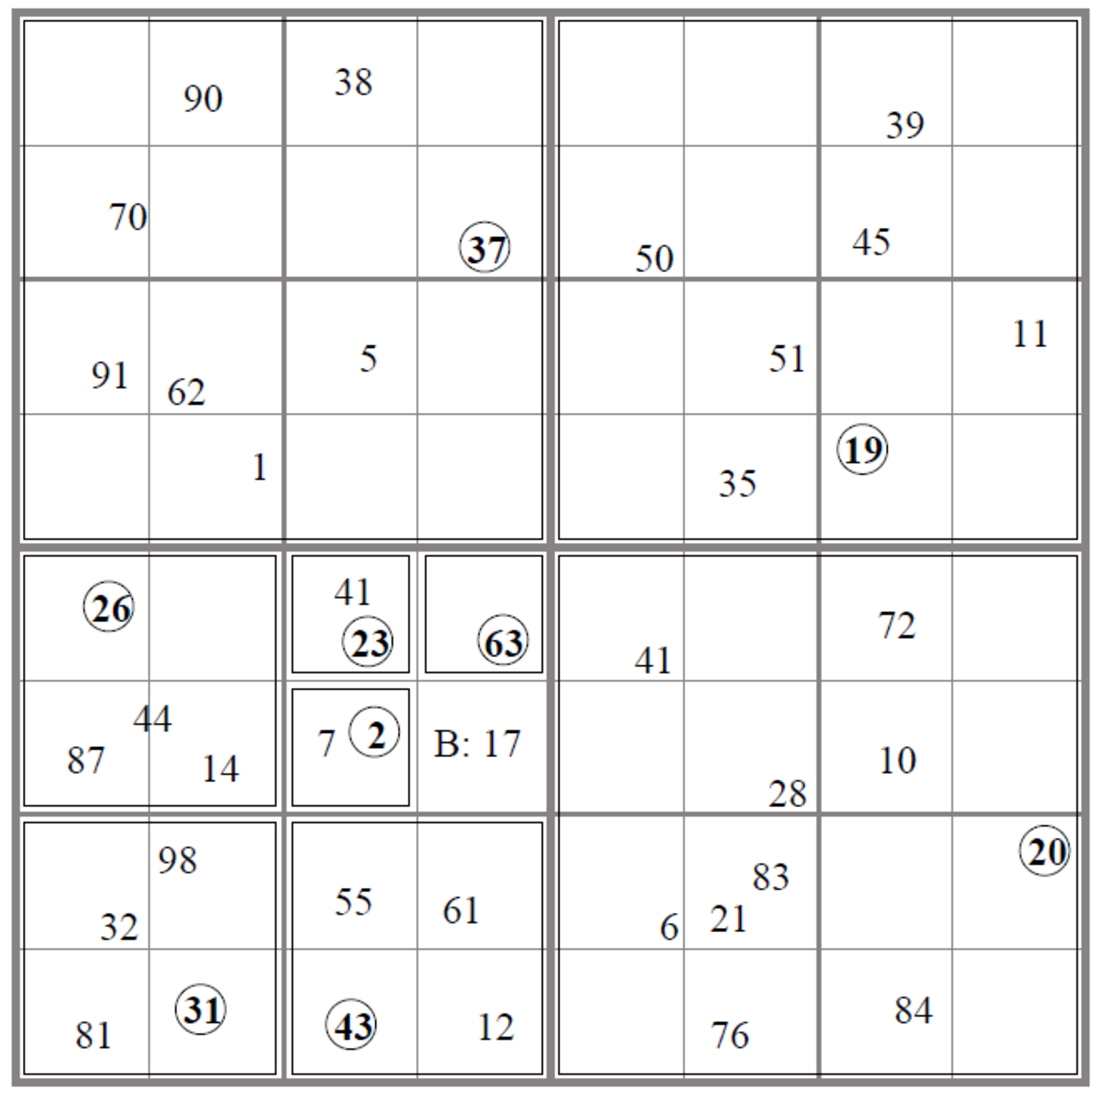
\includegraphics[width=\colwidth]{../../images/external/location_routing/location_service.pdf}
\caption{Hierarchical grid with 4 order-i squares in order-i+1 square.}
\end{figure}

An example of such a system, presented in \cite{Li:2000:SLS:345910.345931}, uses a routing technique in which each node maintains a list of neighbors, found through periodically broadcasted HELLO packets, and forwards a message to the neighbor known to be closest to the destination.
The HELLO messages are broadcast one hop away to extend local neighborhood knowledge.
Each node maintains its location in a number of \emph{location servers}, which are other nodes in the network.
Location servers' occur more densely near a node and less densely farther away in order to decrease inefficiencies for lookups made nearer to the node.

As shown in Figure \ref{fig:location-service}, the geographic space is divided up into hierarchical square regions (each order-2 square is comprised of 4 order-1 squares, the smallest, and so on).
At each level of this hierarchy, a node is chosen as a server within each of the 3 order-i squares external to the one the source node resides in but contained within the order-i+1 square the source resides in. 
The servers are chosen by having an ID closest to the source's, but greater (the ID space is circular).
This is done by initially forwarding the packet to a particular region that the source wants a location server in.
The message is then forwarded locally until the appropriate node within that region is found.
The bootstrapping process involves first finding the order-1 servers, then order-2, etc.

Note that a message should never travel farther than the size of the smallest square in which source and destination are co-located.
In fact, each lookup only takes n steps where the order-n square is the smallest square that source and destination are co-located in.   
Each step in the lookup process brings the query to the best node in the next larger square.          
Each node sends updated information (outside the order-1 square since those are immediate neighbors) periodically.
The number of updates is proportional to the node's speed in order to avoid stale information caused by high mobility.
To handle query failures due to nodes leaving a region, forwarding pointers are left behind, which are piggy-backed on the HELLO messages.

% % % % % % % % % % % % % % % % % % % % % % % % % % % % % % % % % % % % % % % % % %

\section{Greedy Forwarding}

To actually route a message through a network using location information, each router (intermediate node) must know how to forward the packet to the next hop.
The simplest method to accomplish this is for the node to forward the packet to its neighbor who is closest to the destination.
To avoid loops and ensure delivery, the next hop must be closer to the destination than the previous.
However, this can result in a local minimum in which no available neighbors are closer to the destination.
Such a situation, shown in Figure \ref{fig:network-void}, is referred to as a \emph{void}.
Many works, some of which are described below, have proposed solutions to this problem.
This section outlines protocols that use this greedy forwarding paradigm and how they address the problem of voids.

The protocol in \cite{Yu01geographicaland} uses greedy forwarding, but to address holes in the network it uses a learned cost function of forwarding to the destination for each neighbor.  Once a packet reaches the target region, the data is diffused through either recursive geographic forwarding or restricted flooding.  The latter is better in less dense networks.

\begin{figure}
\label{fig:network-void}
\centering
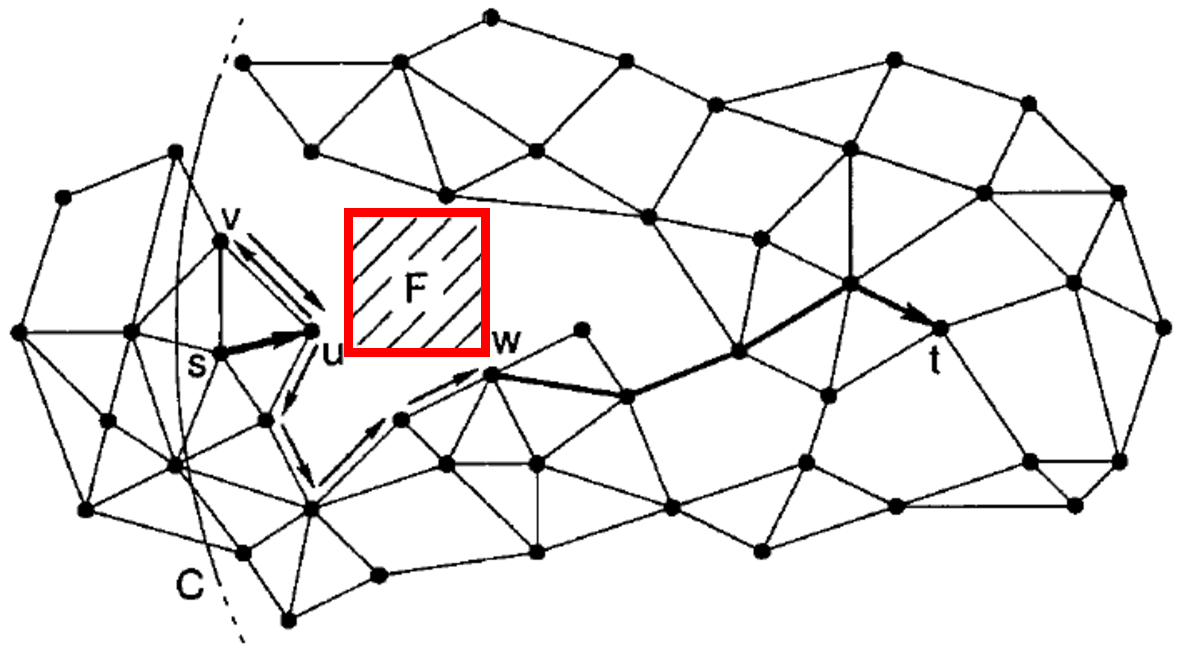
\includegraphics[width=\colwidth]{\imagepath/void}
\caption{A void in a network (roughly centered at F, outlined in red) may disrupt greedy forwarding}
\end{figure}


In \cite{Ko98location-aidedrouting}, the destination (D) is assumed to be in some circular region (representing a margin of error), whose radius is defined based on D's velocity, which is assumed known to all nodes.
Route requests are only forwarded if the node is within this expected zone, so other zones are added to fill gap between the source (S) and D's zones; these are called \emph{request zones}.
A failed request, caused by events such as peers residing outside of the tear-drop shaped expected zones, recover by simply flooding the whole network.
To deliver messages, the following steps are performed:
\begin{itemize}
 	\item Draw a minimum sized rectangle to include the expected zone circle and S
	\item A node only forwards if it is closer than the previous node + $\delta$, where $\delta$ is a configurable parameter (0 in their simulations) to avoid local minima.
\end{itemize}

%Simple random walk models, no waiting in between, varied speeds and distances.
%No transmission errors, or channel contention.
%Increased error seems to have little effect on number of routing packets sent per data packet: likely due to increasing expected zone size for higher error.

The authors also present several possible optimizations to their protocol.
One is to use larger request zones, gradually increasing their size after failures.
Another is adapting the request zone at intermediate nodes if they have better info about location.
They also propose propagating speed/location information by piggybacking on other packets.
Furthermore, intermediate nodes detecting route failures could possibly initialize a local search to decrease request zone size.

A method for multicasting messages to a geographic region is proposed in \cite{749282}.
They define a forwarding zone so that all nodes in that zone will forward a multi-cast packet via flooding to the actual multi-cast region, which is the target region.
These concepts are depicted in Figure \ref{fig:multicast-region}.
They define two schemes for regional multicasting:
\begin{itemize}
\item \textbf{Rectangle:} the source defines a rectangular region and nodes within it will forward the message .
They include a parameter, $\delta$, to increase the size of the rectangle so that the source and multi-cast region are not on the very edges of the rectangle.          
\item \textbf{Non-explicit:} the source includes information about the multi-cast region and source's location.
Intermediate nodes forward the packet if they are at most $\delta$ (a different parameter from the first scheme) farther away from the destination region's geographic center than the previous hop.
\end{itemize}
Their simulation results show that the first scheme is generally more accurate (in terms of the number of nodes in the multicast region that receive the message).
They found that the scheme's accuracy is comparable with that of multicast flooding, while having less overhead.

\begin{figure}
\label{fig:multicast-region}
\centering
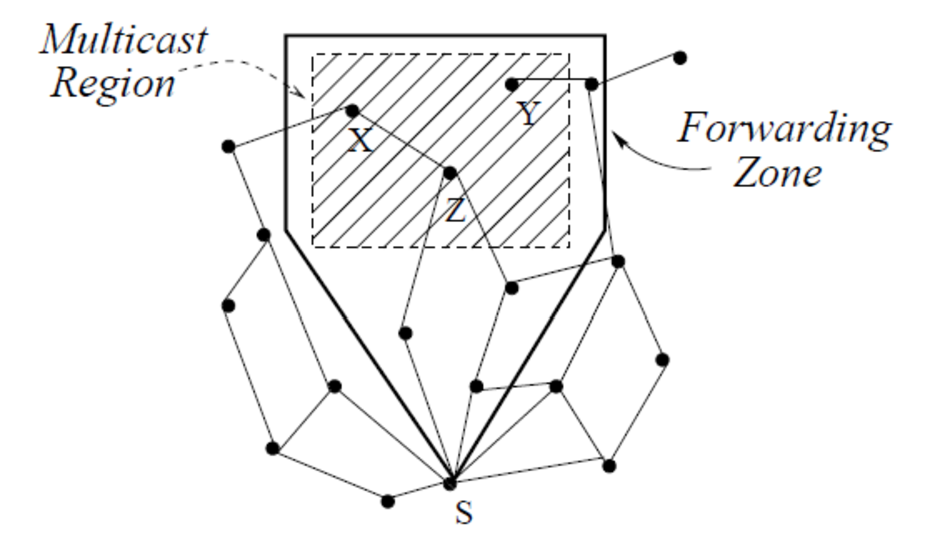
\includegraphics[width=\colwidth]{\imagepath/geocast_region}
\caption{Depiction of multicast region and forwarding zone}
\end{figure}

The concept of \emph{mobicast} is presented in \cite{Huang2005}.
It consists of delivering messages to a moving geographic region.
Initially, packets are forwarded as soon as possible (ASAP) when a node is within or adjacent to the current delivery zone.
If it is not, the node will enter timed forwarding and will wait to forward the message until it or one of its neighbors is within the delivery zone, taking expected latency into account.
This is referred to as just in time (JIT) forwarding.
%To aintaining a spatial neighborhood as the set of nodes in all faces adjacent to the node except itself.


% % % % % % % % % % % % % % % % % % % % % % % % % % % % % % % % % % % % % % % % % %

\section{Geometric Routing}

To address some of the shortcomings of greedy forwarding, several works have proposed techniques for routing based on geometric graphs.
Such strategies make use of the structural properties of a network to make guarantees on efficiency, delivery time, etc.
One of the first to do so is \cite{Kranakis99compassrouting}, which introduced \emph{compass routing}.
In this scheme, a graph is constructed to represent the network in which each vertex is a node and an edge represents a pair of nodes' ability to communicate with each other.
When a node receives a packet along an ingress link, it forwards it along the egress link next in counter-clockwise order from the ingress link, as shown in Figure \ref{fig:right-hand-rule}.
This is sometimes referred to as the \emph{right-hand rule} or \emph{face routing}.

\begin{figure}
\label{fig:right-hand-rule}
\centering
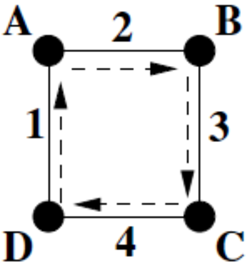
\includegraphics[width=\colwidth]{\imagepath/right_hand_rule}
\caption{The right-hand rule: forward packet along next counter-clockwise edge. Analogous to following the right hand wall in a maze.}
\end{figure}

Because compass routing requires a planar graph to perform correctly, \cite{Kim:2005:GRM:1251203.1251219} proposed a protocol that eliminates cross-links (links between two pairs of nodes that cross).
They use probing and the right-hand rule of traversing faces in order to create a planar graph and facilitate geographic routing using face following.

Several works use a hybrid of greedy distance-based and compass routing.
In \cite{Kuhn2003}, a message explores the face within a bounded region, enlarging that region if it reaches the end and must turn back before reaching destination.
Maintain a counter of how many nodes closer and farther they reach when in face routing mode.
They also show that a route along a Clustered Backbone Graph, in which regular nodes cluster around nearby backbone routing nodes, is longer than the optimal path by a constant factor only.
Their research also found that they must explore complete boundary of current face in order to remain asymptotically optimal.
Therefore, a node cannot simply switch back to greedy when the message finds a closer node.
%Formally prove that it is worst-case asymptoticaly optimal.

A similar technique is used in \cite{Karp2000}, in which nodes greedily routes packets such that each hop becomes progressively closer to destination.
They address local minima by switching to compass routing mode.

% % % % % % % % % % % % % % % % % % % % % % % % % % % % % % % % % % % % % % % % % %

\section{Trajectory-based Routing}

% % % % % % % % % % % % % % % % % % % % % % % % % % % % % % % % % % % % % % % % % %
Several recent studies ( \cite{Niculescu2003} \cite{Niculescu2004} \cite{Yuksel2006} ) had concentrated on Trajectory-based Routing (TBR) which serves as a middle ground between source-based routing and greedy forwarding. The sender node would encode trajectory to packets upon transmission (shown in Figure \ref{fig:trajectory}), whereas the intermediate nodes would perform greedy forwarding based on the trajectory information it decodes in the 
packets that have been received. TBR has been attracting attentions in the academic field for the following reasons. First of all, the very idea of TBR is well-suited for overlay routing schemes since trajectory information could be not obtained directly from the network layer. For application-based overlay networks, TBR enables
the application layer provides the trajectory information for routing. Moreover, for scenarios like geo-routing protocols that specify certain geological area on route are needed when emergency occurs, TBR would serve this purpose better than other routing schemes. Last but not least, TBR is not only designed for wireless mesh network but also 
large scale wired network, which suite the purpose of our research.

\begin{figure}
\label{fig:trajectory}
\centering
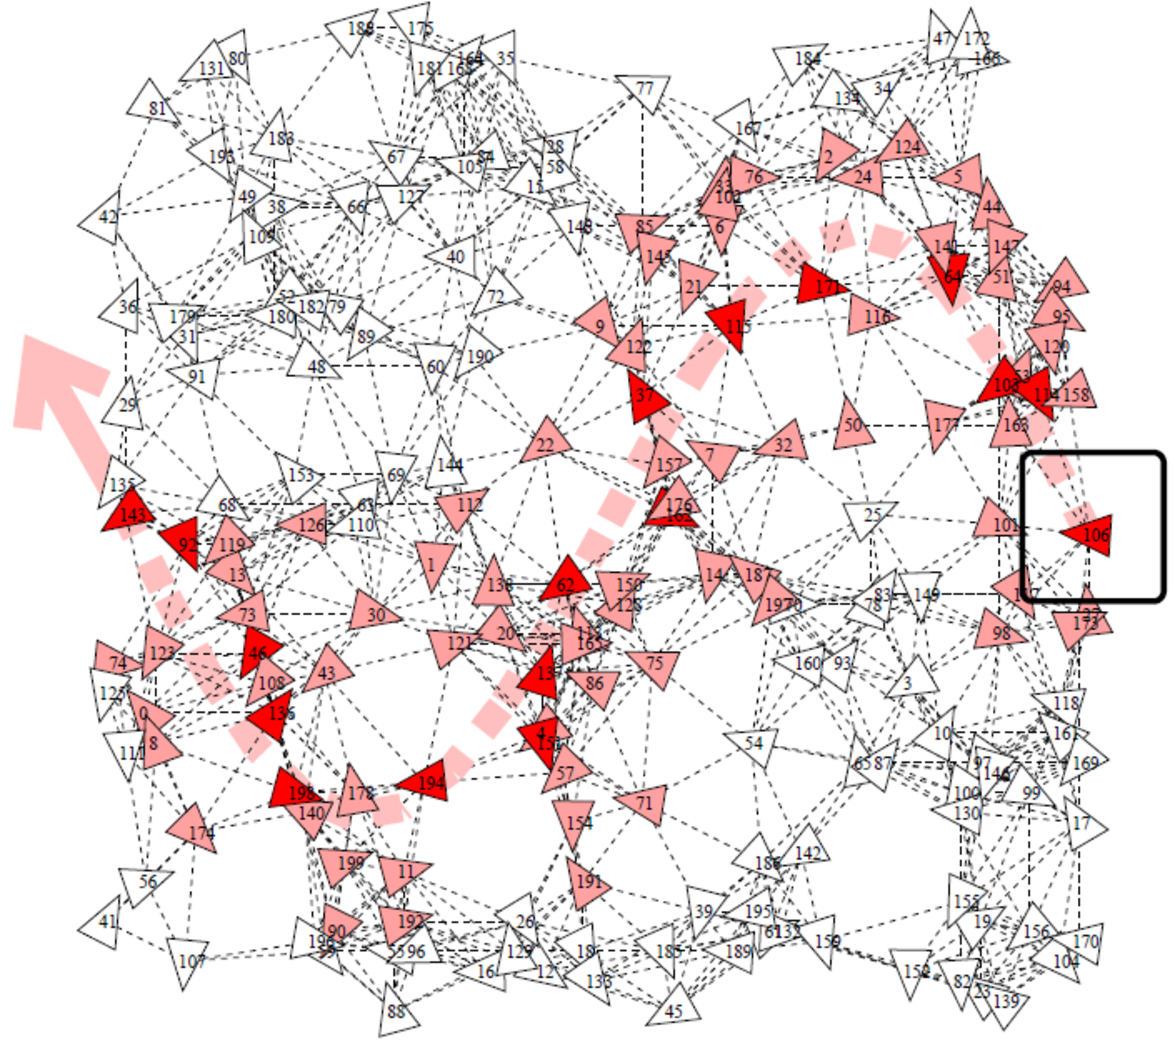
\includegraphics[width=\colwidth]{\imagepath/trajectory}
\caption{Forwarding along a trajectory}
\end{figure}

\section{Agent/Agent-less Zone Forwarding}

% % % % % % % % % % % % % % % % % % % % % % % % % % % % % % % % % % % % % % % % % %
Important earlier papers like \cite{Basagni1998} had laid out several import features regarding geocast protocol design, one of which is forwarding zone. In order to avoid flooding the whole ad hoc network, protocols like \cite{Basagni1998}, \cite{Camp2003}, \cite{Liao} and so on devide the network into several Forwarding Zones (FZ). Geocast messages would 
only be flooded within the given FZ so as to reduce the oervall network traffic. The shape of the FZ could depend on what the specific protocol demands, it could be triagular, rectangular or something else. However, the protocols utilizing FZ is different on how to forward packets. Protocols like \cite{Basagni1998} utilize basic greedy forwarding within
the FZ, i.e. the node will flood its all one-hop neighbours within the FZ. On the other hand, protocols like \cite{Liao} deploy an election scheme. Every grid (FZ) would elect an agent to forward the packet to other grids (FZs). The agent-based forwarding would reduce some redundancy caused by agentless flooding, however the control overhead 
introduced in the election procedure cannot be ignored.

% % % % % % % % % % % % % % % % % % % % % % % % % % % % % % % % % % % % % % % % % %

\section{Clustering}

Clustering is an important issue in location-based routing, especially in geo-routing. The intermediate nodes are organized into clusters (or zones, grids) to perform forwarding.
This improves efficiency and scalability, especially important for larger and more mobile networks.

A modified AODV with expected transmission count (ETX) instead of minimum hop count is proposed in \cite{Al-Rabayah2010}.
Intermediate nodes can repair routes locally instead of notifying about their failure.
The data packets are buffered to destination until a suitable path is found, which is done by either looking up if a path exists through one of their neighbors or by flooding the route repair packet to all neighbors and awaiting a reply.

Moreover, the protocol proposed in the paper is designed to gracefully degrade to reactive flooding algorithm in the absence of location information by simply flooding if no neighbors are deemed closer to the destination.
This may occur because they are actually farther away or because their location information isn't available.
The former case can arise when there is a void in the network and the latter if the node has no GPS device or it is malfunctioning.

Two levels of routing, intra- and inter-zone, are proposed in \cite{779923}.
Intra-zone routing is done proactively (like link state routing protocols).
An inter-zone clustering protocol runs and updates with information about inter-zone links periodically.
However, the paper does not  provide information about the exact location of destination within a zone.
Instead, the message is routed to that zone and then a node within it handles delivery to the final destination.

GRID, which is proposed in \cite{Liao01grid:a}, is a reactive routing protocol where a geographic region is divided into logical grids, each a square, with an elected leader of each grid.
It avoids broadcast storms since only the leader of each grid handles routing (density-agnostic). 
However as the number of grids approaches the number of hosts, it returns to normal flooding.
Each grid is the same size and is chosen based on transmission range and whether the source in a grid can talk to 4 or 8 of the neighboring grids, with destination gateways preferably in the center or anywhere in those grids.
There is a trade-off between the sizes as too big will make it hard to reach the next grid neighbor whereas too small results in higher overhead and a decreased probability of a node being available to fill a gateway position.
For routing, GRID employs a zone-based version of AODV, where route requests have a range parameter to define a search area.
The zones could be confined by 4 shapes: 
\begin{itemize}
\item Rectangle
\item Bar from source to destination with some width
\item Fan with angle and radius
\item Overlap of 2 fans
\end{itemize}

Gateways  are chosen as the node closest to center of zone. A node would remain as a gateway until leaving the zone.
If a node hasn't heard from a gateway in a while, it will broadcast a packet: the gateway replies if still there and other nodes that are closer to center reply so that after some time a new gateway is chosen if the old one left.
Because broadcast is unreliable, if two gateways exist, one will silently step down when it hears a GATE packet from a closer gateway.
GATE packets every 10 seconds.

A subset of nodes that are GPS-enabled form a backbone in \cite{Zaruba2003}, handling routing and proactively exchanging link information with each other.
Other nodes belong to the zone surrounding one of these G-nodes.
They assume the same location as the nearby G-node, but may be a few hops away.
The virtual backbone is formed by a root G-node sending messages to nearby zones until all are a part of the virtual backbone, as shown in Figure \ref{fig:labar-routing}.
G-nodes translate IP addresses to geographic locations, determines a vector towards the destination, and instructs the source node how to route the message to a nearby zone closest to this vector.
If this forwarding fails, the source is notified and the packet is forwarded along the backbone.

\begin{figure}
\label{fig:labar-routing}
\centering
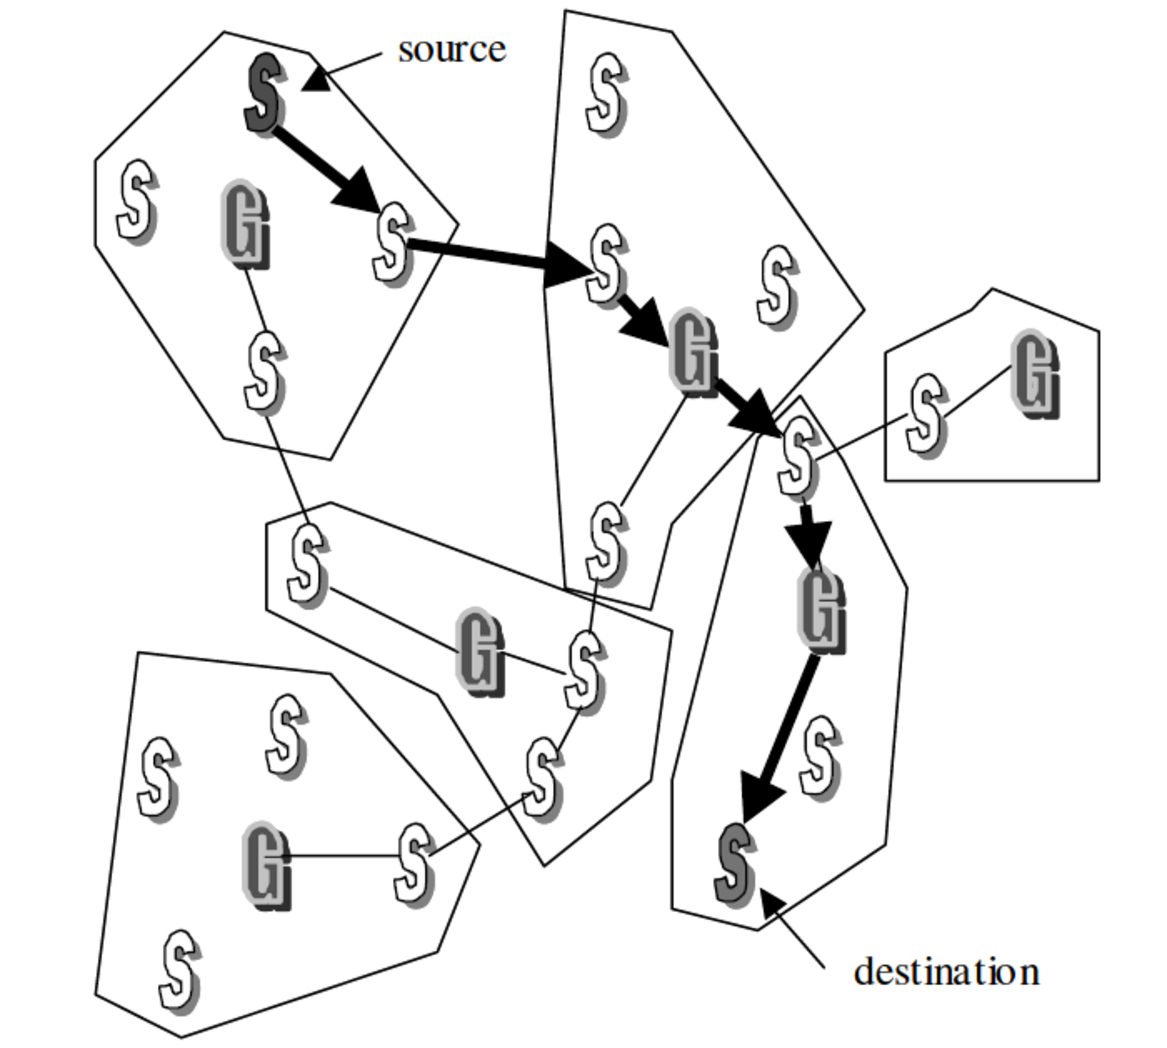
\includegraphics[width=\colwidth]{\imagepath/labar.pdf}
\caption{Routing in LABAR}
\end{figure}

In \cite{Rodoplu}, node pairs are associated with \emph{relay regions}, which are the nodes around the sender that are more energy efficient to send through than directly to the receiver.
The \emph{enclosure} of a node is then defined as all of the relay regions it can reach.  The protocol establishes a sub-network that will require less power and has fewer nodes for reaching some destination.
This is accomplished by first creating a sparse graph representing all of the enclosures in each transmitting node in the network, which is done through local computation.  This graph contains globally optimal links (in terms of energy), which are then fed into a distributed Bellmann-Ford algorithm with power consumption as the cost metric.  This algorithm is self-configuring and can respond to failures and mobile nodes.  It was originally designed for mobile p2p networks, but is highly applicable to sensor networks as well.

% % % % % % % % % % % % % % % % % % % % % % % % % % % % % % % % % % % % % % % % % %

\section{Wired Networks}

While location-based routing in wired networks has predominately been overlooked in the literature, a few works have proposed various such techniques.
They typically address delivering messages to specific regions or avoiding geographically-correlated failures in the network.

In \cite{Navas1997}, the authors proposed, in an IETF RFC, an infrastructure for geographic multicast.
They proposed several possible approaches:
\begin{itemize}
\item Geographic routers
\item Geographic multi-cast
\item Domain Name System
\end{itemize}

They implemented the first approach, geographic routers, for routing messages to specific locations.
Regions are defined as points, circles, or polygons consisting of points.
The system consists of 3 main components:
\begin{itemize}
\item GeoRouter - routes packets and is responsible for some region
\item GeoNode - handles storing/forwarding data to the smaller region it is responsible for
\item GeoHost - the actual processes running on end hosts 
\end{itemize}

GeoRouters use a caching mechanism with timeouts indexed by the hash of the message ID.
They determine their service area by finding the convex hull of all the children's service areas, which are polygons, in order to avoid inefficiencies introduced by concave polygons and those with holes.
If a message is destined for an area a router doesn't serve, it forwards the message to its parent router.
Experimental results reveal some improvements in routing, mostly due to more efficiently checking polygons' intersections.

In \cite{Kim2010}, the effects of geographically-correlated failures on overlay-based data dissemination are considered.
Overlay neighbors are chosen to minimize the number of routers along the paths that are closer than some threshold distance.
The authors base this choice on the intuition that regional failures are more likely to affect multiple nodes in close proximity, as shown in Figure \ref{fig:geo-failure} and so the path choices should be more diverse.

\begin{figure}
\label{fig:geo-failure}
\centering
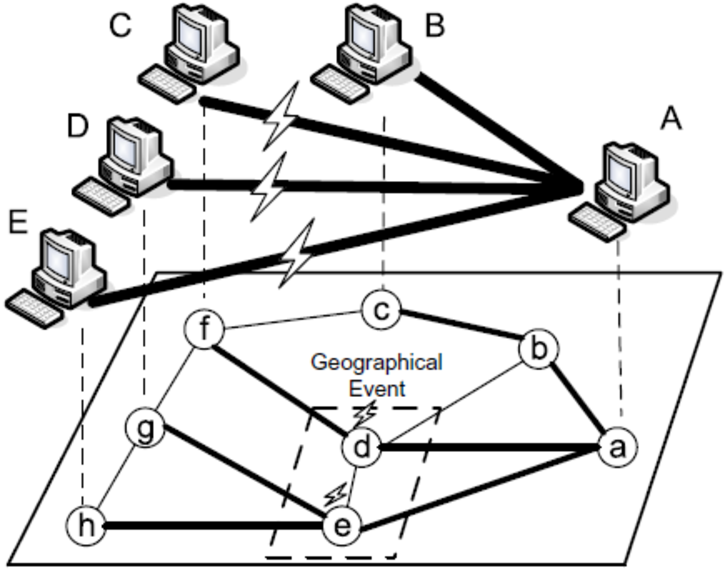
\includegraphics[width=\colwidth]{\imagepath/geo_failures_kyungbaek.pdf}
\caption{Different overlay links may share the same underlay links/nodes}
\end{figure}

Contrary to \cite{Kim2010}, the authors in \cite{Benson2013} consider that the underlying network topology may be unknown or inaccurate.
They study the scenario of delivering data from a seismic sensor network during a powerful earthquake that may damage telecommunications infrastructure.
To route around a perceived failure, they propose a heuristic, depicted in Figure \ref{fig:orthogonal-path}, that chooses an intermediary overlay hop as being far away from the straight line path from the reporting sensor to the server it wishes to contact.
The intuition here is that the failure is likely nearby the node or along the path to the server and so avoiding that path as much as possible by routing along a trajectory angled away from it should improve the chance of data delivery.

\begin{figure}
\label{fig:orthogonal-path}
\centering
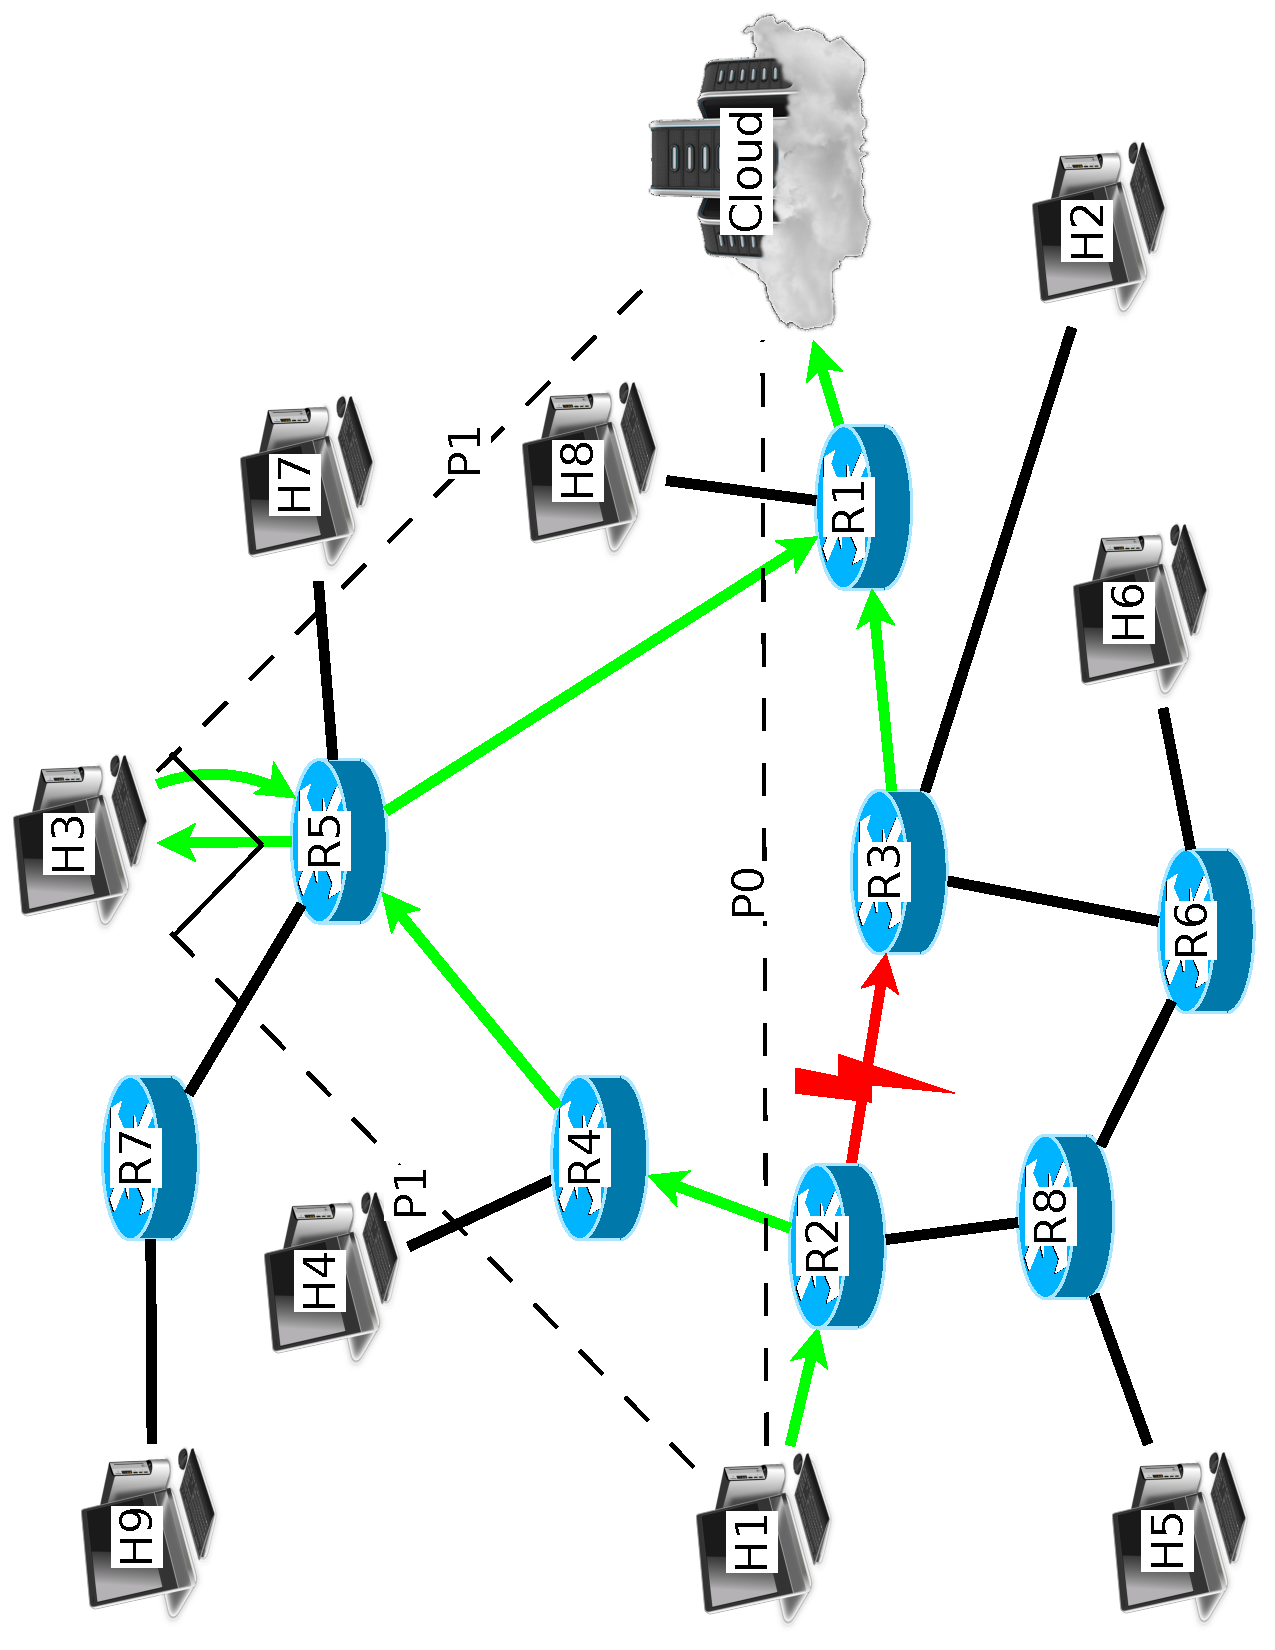
\includegraphics[width=\colwidth,angle=-90]{\imagepath/../../diagrams/angular_path.pdf}
\caption{To avoid the failure along the path to the server, packets are routed along a trajectory angled away from that straight line path}
\end{figure}

% % % % % % % % % % % % % % % % % % % % % % % % % % % % % % % % % % % % % % % % % %

\section{Conclusion}
\label{conclusion}
As what are illustrated above, several studies have been done regarding location-based routing in recent years, and progress have been made in many aspects. 

It is worth noting that a large amount of the researches have dealt with the wireless network. It is important to identify the differences between wireless and wired network. For routing protocols that involve wireless network, there are several aspects that need to be taken into consideration
such as the hop count, the constant changing of topology, the hidden node effect, the high transmission loss rate and so on. However these limitations are not always obstacles. For example, when an overlay routing scheme built on a wired network is considered, certain methods involving large packet overhead and hop count, that could not be used in wireless network due to the limits mentioned before, could become useful.  Admittedly, problems like overhead introduced by node election, network convergence, loop-avoidance and so on, are universal regardless wired or wireless network. 

The location-based routing is very helpful in dealing with overlay networks, since location information usually could not be obtained from network layer. Location information-driven geo-routing would provide a more physical-matched topology to enhance the ability of network recovery.
Furthermore, it enables a host of services such as regionally targeted broad/multicasting, spatial querying, and more efficient routing and querying by exploiting nearby nodes/servers.
While many such applications will be aimed at wireless environments, as the literature shows they already are, we anticipate an increase in the number of works focusing on location routing in wired networks in the coming years, especially as individuals and organizations continue to further consider the impact of large-scale disasters on our increasingly techno-centric societies.
% use section* for acknowledgement
%\section*{Acknowledgment}



% An example of a floating figure using the graphicx package.
% Note that \label must occur AFTER (or within) \caption.
% For figures, \caption should occur after the \includegraphics.
% Note that IEEEtran v1.7 and later has special internal code that
% is designed to preserve the operation of \label within \caption
% even when the captionsoff option is in effect. However, because
% of issues like this, it may be the safest practice to put all your
% \label just after \caption rather than within \caption{}.
%
% Reminder: the "draftcls" or "draftclsnofoot", not "draft", class
% option should be used if it is desired that the figures are to be
% displayed while in draft mode.
%
%\begin{figure}[!t]
%\centering
%\includegraphics[width=\colwidth]{myfigure}
% where an .eps filename suffix will be assumed under latex, 
% and a .pdf suffix will be assumed for pdflatex; or what has been declared
% via \DeclareGraphicsExtensions.
%\caption{Simulation Results}
%\label{fig_sim}
%\end{figure}

% Note that IEEE typically puts floats only at the top, even when this
% results in a large percentage of a column being occupied by floats.


% An example of a double column floating figure using two subfigures.
% (The subfig.sty package must be loaded for this to work.)
% The subfigure \label commands are set within each subfloat command, the
% \label for the overall figure must come after \caption.
% \hfil must be used as a separator to get equal spacing.
% The subfigure.sty package works much the same way, except \subfigure is
% used instead of \subfloat.
%
%\begin{figure*}[!t]
%\centerline{\subfloat[Case I]\includegraphics[width=2.5in]{subfigcase1}%
%\label{fig_first_case}}
%\hfil
%\subfloat[Case II]{\includegraphics[width=2.5in]{subfigcase2}%
%\label{fig_second_case}}}
%\caption{Simulation results}
%\label{fig_sim}
%\end{figure*}
%
% Note that often IEEE papers with subfigures do not employ subfigure
% captions (using the optional argument to \subfloat), but instead will
% reference/describe all of them (a), (b), etc., within the main caption.


% An example of a floating table. Note that, for IEEE style tables, the 
% \caption command should come BEFORE the table. Table text will default to
% \footnotesize as IEEE normally uses this smaller font for tables.
% The \label must come after \caption as always.
%
%\begin{table}[!t]
%% increase table row spacing, adjust to taste
%\renewcommand{\arraystretch}{1.3}
% if using array.sty, it might be a good idea to tweak the value of
% \extrarowheight as needed to properly center the text within the cells
%\caption{An Example of a Table}
%\label{table_example}
%\centering
%% Some packages, such as MDW tools, offer better commands for making tables
%% than the plain LaTeX2e tabular which is used here.
%\begin{tabular}{|c||c|}
%\hline
%One & Two\\
%\hline
%Three & Four\\
%\hline
%\end{tabular}
%\end{table}


% Note that IEEE does not put floats in the very first column - or typically
% anywhere on the first page for that matter. Also, in-text middle ("here")
% positioning is not used. Most IEEE journals/conferences use top floats
% exclusively. Note that, LaTeX2e, unlike IEEE journals/conferences, places
% footnotes above bottom floats. This can be corrected via the \fnbelowfloat
% command of the stfloats package.



% trigger a \newpage just before the given reference
% number - used to balance the columns on the last page
% adjust value as needed - may need to be readjusted if
% the document is modified later
%\IEEEtriggeratref{8}
% The "triggered" command can be changed if desired:
%\IEEEtriggercmd{\enlargethispage{-5in}}

% references section

% can use a bibliography generated by BibTeX as a .bbl file
% BibTeX documentation can be easily obtained at:
% http://www.ctan.org/tex-archive/biblio/bibtex/contrib/doc/
% The IEEEtran BibTeX style support page is at:
% http://www.michaelshell.org/tex/ieeetran/bibtex/
\bibliographystyle{IEEEtran}
% argument is your BibTeX string definitions and bibliography database(s)
\bibliography{IEEEabrv,location_routing_survey}


% that's all folks
\end{document}


